\chapter{Evaluation}
\label{chap:evaluation}

In this chapter we evaluate the performance of our model and novel font selection interface. Our Model Evaluation section includes a quantitative analysis of our model encodings, calculating the average pairwise distances of font groups in our model space according to the Google Fonts typeface categories discussed in Section \ref{font-selection-innovation}. In our User Evaluation section, we test our font selection interface against two alternate font selection tools with a small user study involving a font matching task and an open-ended qualitative evaluation. While the user evaluation certainly evaluates the usability and effectiveness of our selection interface, the model space itself---how accurately the model encodes typeface style---also affects the usability of the tool. Therefore, this user evaluation quantifies the combined effectiveness of the model encodings and the selector interface together.

\section{Model Evaluation} \label{model-eval}

We evaluate our models by measuring the average pairwise distances between fonts within each of the typeface style categories recently introduced by Google Fonts (see Section \ref{font-selection-innovation}), normalized against the overall average pairwise distance in the model space. While these categories are inherently subjective and have some inaccuracies (as previously discussed) they provide a useful grouping which is auxiliary to our model training and therefore can be used to evaluate our model encodings.

\begin{longtable}{|l|r|r|r|r|}
\caption{Average pairwise Euclidean distance between style encodings grouped by Google Fonts categories, normalized relative to the average pairwise distance between all fonts in model space. Distances less than one (closer than average) are bolded. Abbreviated from Table \ref{tab:category-distances} (Appendix).}
\label{tab:category-distances-short} \\
\hline
\textbf{Category} & \textbf{Autoencoder} & \textbf{Style Transfer} & \textbf{Sriv. C64} & \textbf{Sriv. Full} \\
\hhline{|=====|}
average category distance & 1.318 & 1.337 & \textbf{0.952} & \textbf{0.769} \\
\% categories beat average & 34.8\% & 31.8\% & 59.1\% & 98.5\% \\
\hhline{|=====|}
\endfirsthead

\multicolumn{5}{c}{{Table \thetable\ continued from previous page}} \\[0.5em]
\hline
\textbf{Category} & \textbf{Autoencoder} & \textbf{Style Transfer} & \textbf{Sriv. C64} & \textbf{Sriv. Full} \\
\hline
\endhead

\hline \multicolumn{5}{r}{{Continued on next page}} \\
\endfoot

\hline
\endlastfoot

appearance-art-deco       & 1.728          & 1.337          & 1.184          & \textbf{0.780} \\
appearance-art-nouveau    & \textbf{0.453} & \textbf{0.737} & \textbf{0.783} & \textbf{0.706} \\
appearance-blackletter    & \textbf{0.698} & \textbf{0.956} & \textbf{0.956} & \textbf{0.921} \\
appearance-blobby         & 1.198          & 1.276          & \textbf{0.880} & \textbf{0.657} \\
appearance-distressed     & 1.489          & 1.278          & 1.057          & \textbf{0.698} \\
\hline
\multicolumn{5}{|c|}{$\cdots$} \\
\hline
serif-fatface             & 2.478          & 2.896          & 1.082          & \textbf{0.755} \\
serif-humanist            & \textbf{0.628} & \textbf{0.545} & \textbf{0.873} & \textbf{0.841} \\
serif-modern              & \textbf{0.794} & \textbf{0.596} & \textbf{0.847} & \textbf{0.889} \\
serif-old-style           & \textbf{0.522} & \textbf{0.753} & \textbf{0.695} & \textbf{0.814} \\
serif-slab                & 1.582          & 1.347          & 1.117          & \textbf{0.845} \\
serif-transitional        & \textbf{0.551} & \textbf{0.667} & \textbf{0.732} & \textbf{0.954} \\

\end{longtable}

Table \ref{tab:category-distances-short} displays representative results from this evaluation. Each row contains data for a different Google Fonts category, and the four columns represent our four models. (\textbf{Sriv.\ C64} is the Srivatsan model trained only on the Capitals64 dataset, while \textbf{Sriv.\ Full} is the Srivatsan model trained on our full dataset.) Since our distance scores are normalized, values less than one (shown in bold) represent categories whose typeface encodings are closer than the model average, suggesting that salient aspects of the category's style are captured in the model encodings.

We find that the Srivatsan model, trained on the smaller Capitals64 dataset, outperforms both the Autoencoder and Style Transfer models, with a greater number of Google Fonts categories having a lower average distance between fonts than the overall pairwise average ($n=39$), and the average distance score across all the categories slightly lower than the overall average (0.952). However, when trained on our full dataset---including Capitals64, Google Fonts, and the preinstalled fonts from macOS---the Srivatsan model performs even better, with 65 of the Google Font categories having a closer-than-average distance score---all but one---and an average distance score across all the categories of 0.769, much lower than the average pairwise encoding distance.

% my own figure
\begin{figure}[p]
    \centering
    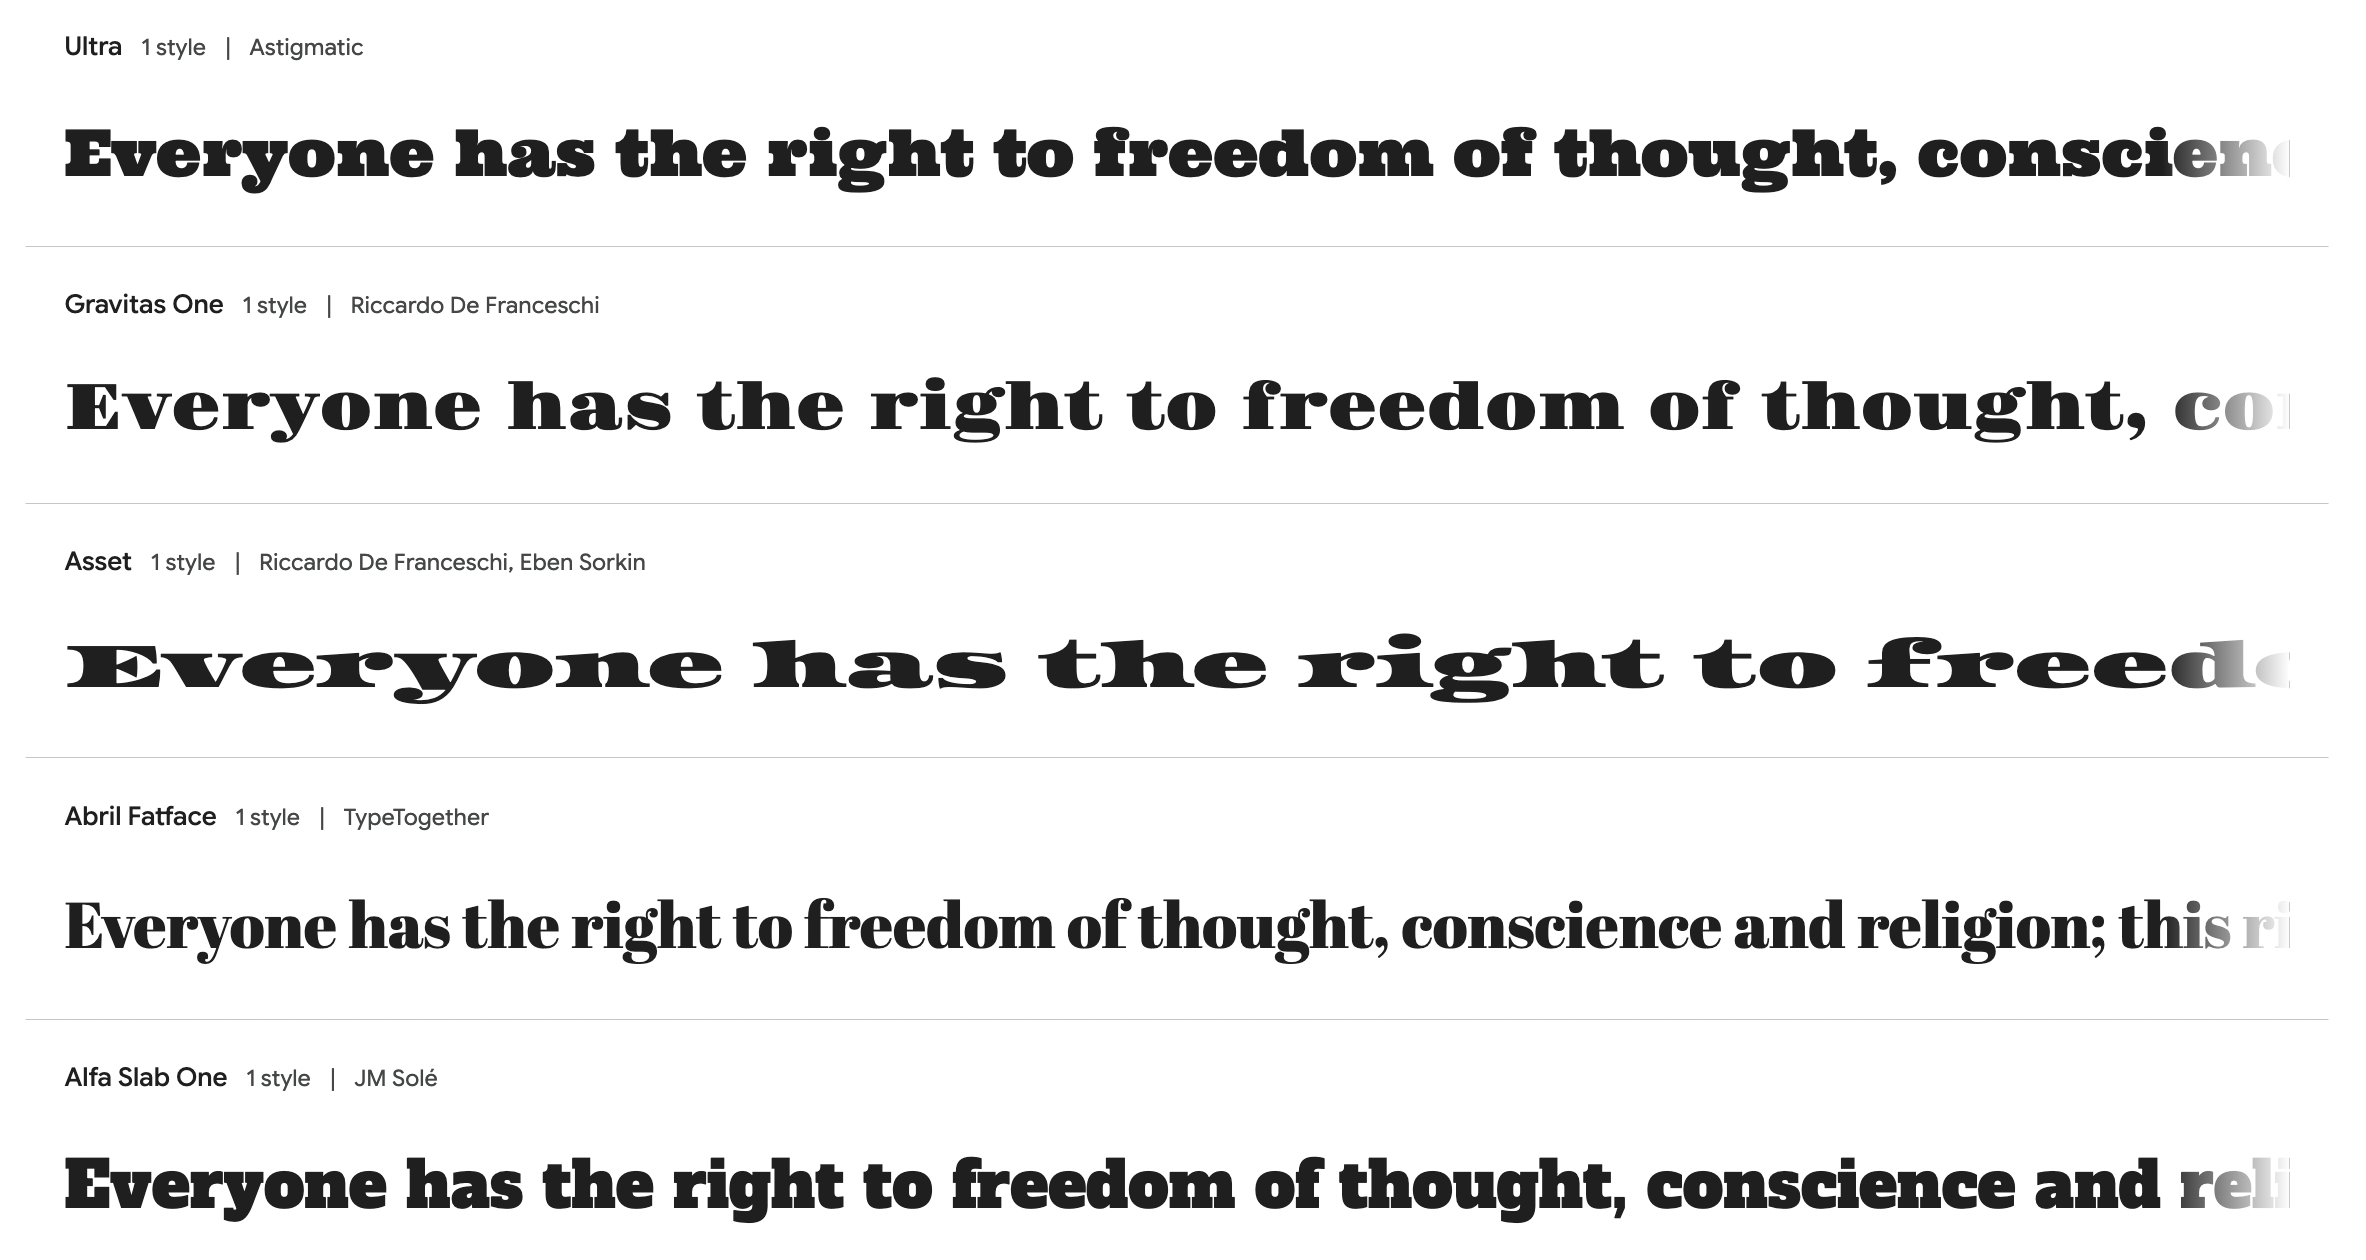
\includegraphics[width=\textwidth]{images/serif-fatface.png}
    \caption{Selection of fonts in the Google Fonts serif-fatface category}
    \label{fig:serif-fatface}
\end{figure}

% my own figure
\begin{figure}[p]
    \centering
    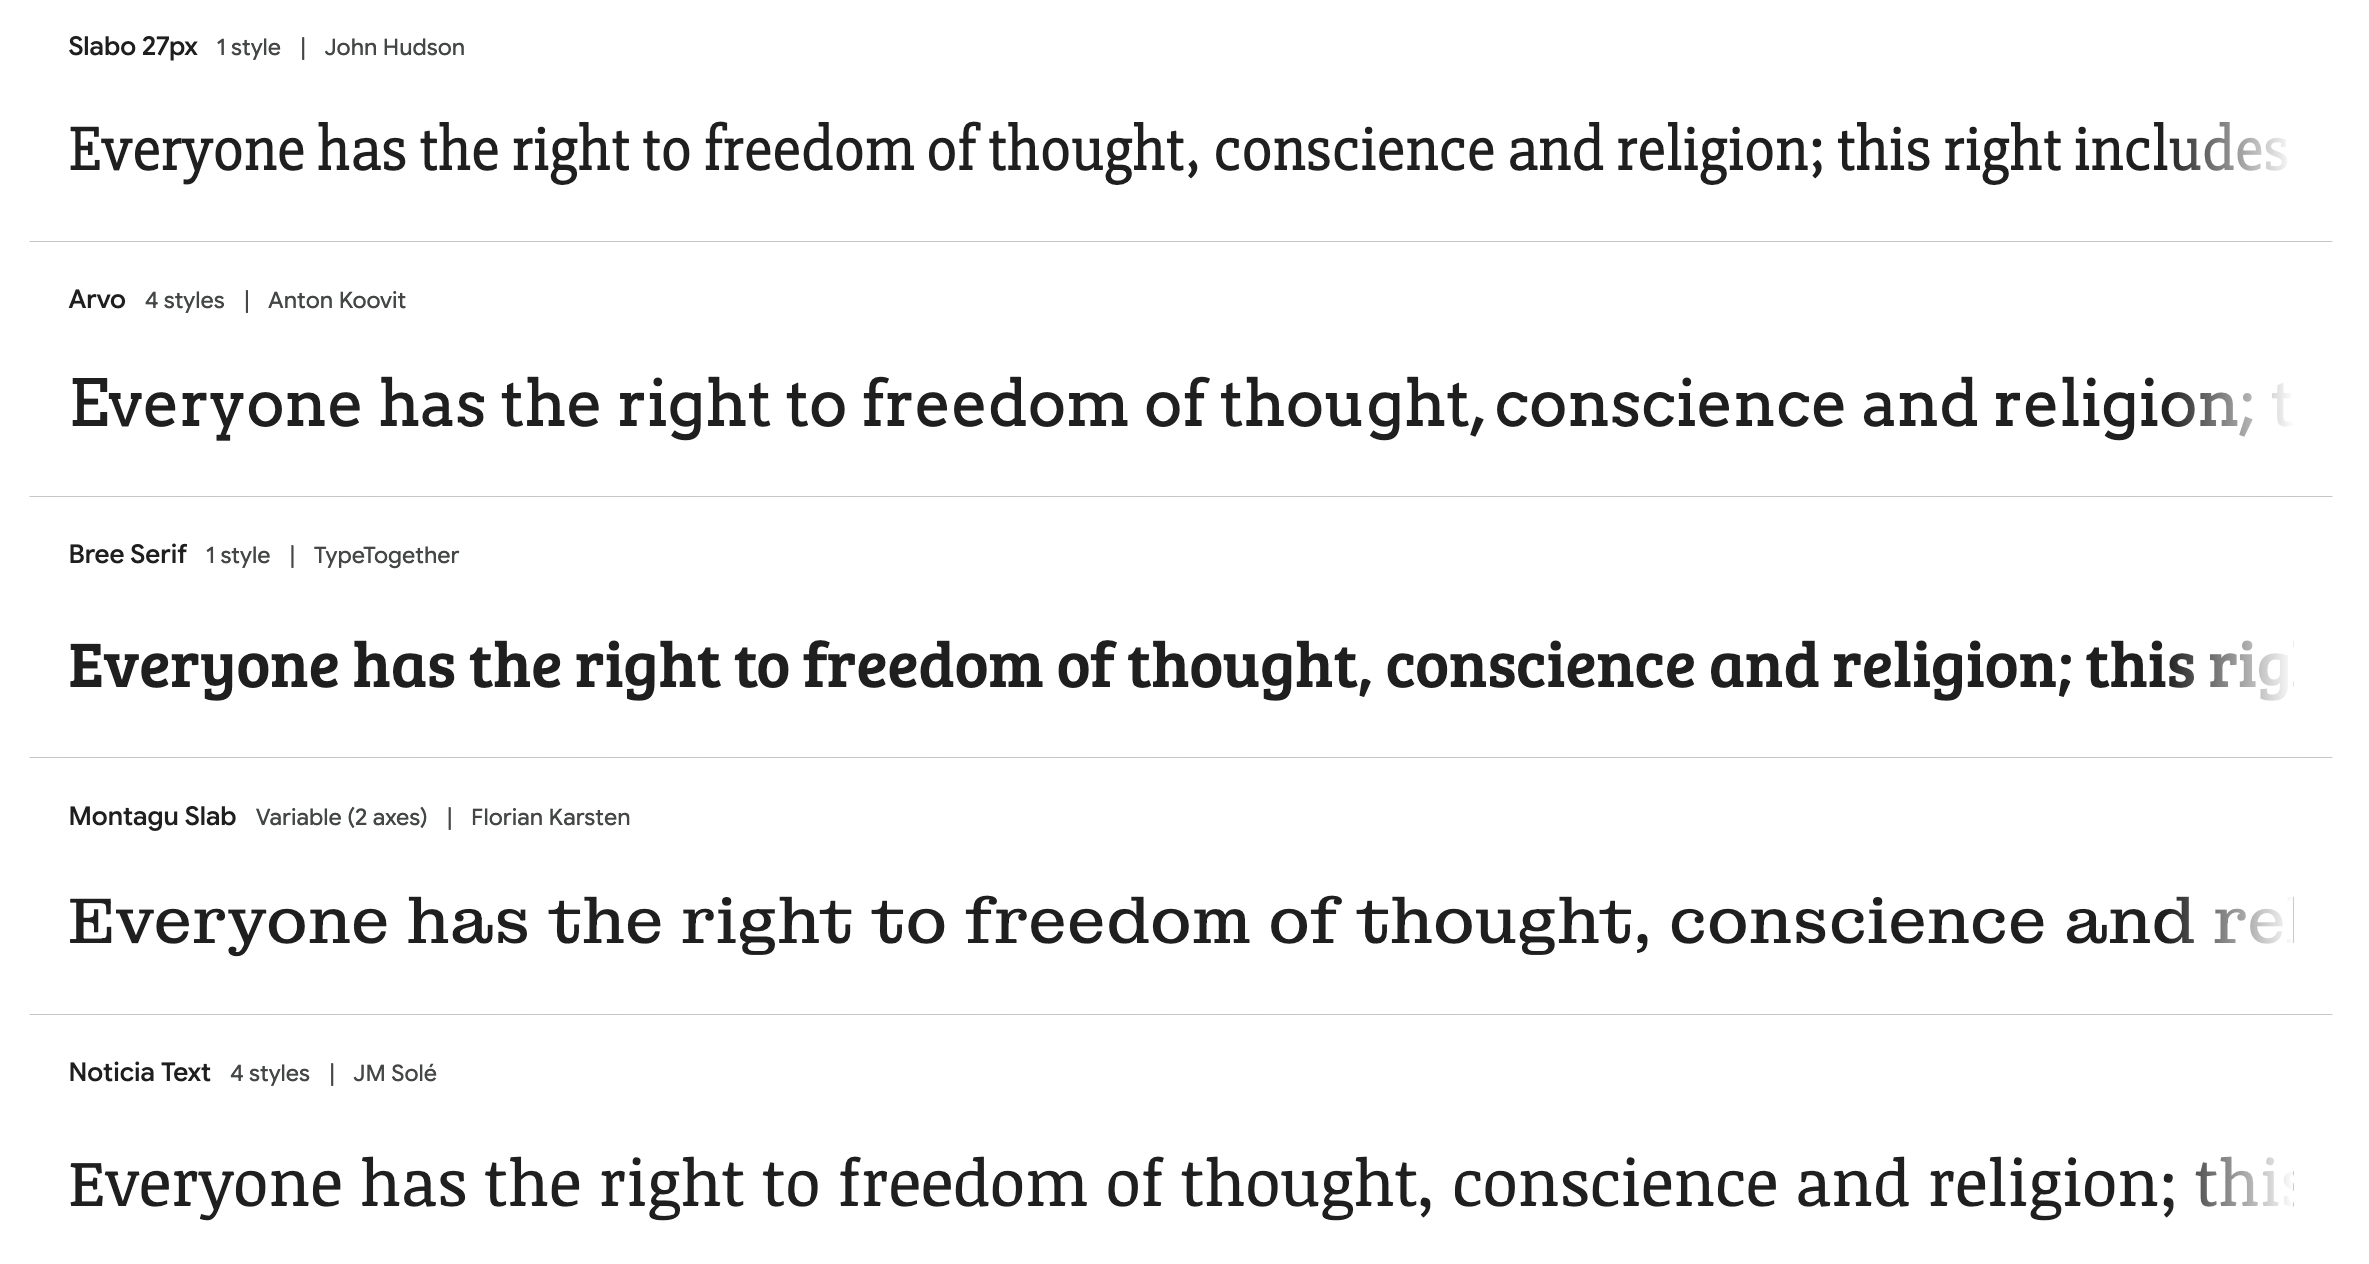
\includegraphics[width=\textwidth]{images/serif-slab.png}
    \caption{Selection of fonts in the Google Fonts serif-slab category}
    \label{fig:serif-slab}
\end{figure}

% my own figure
\begin{figure}[p]
    \centering
    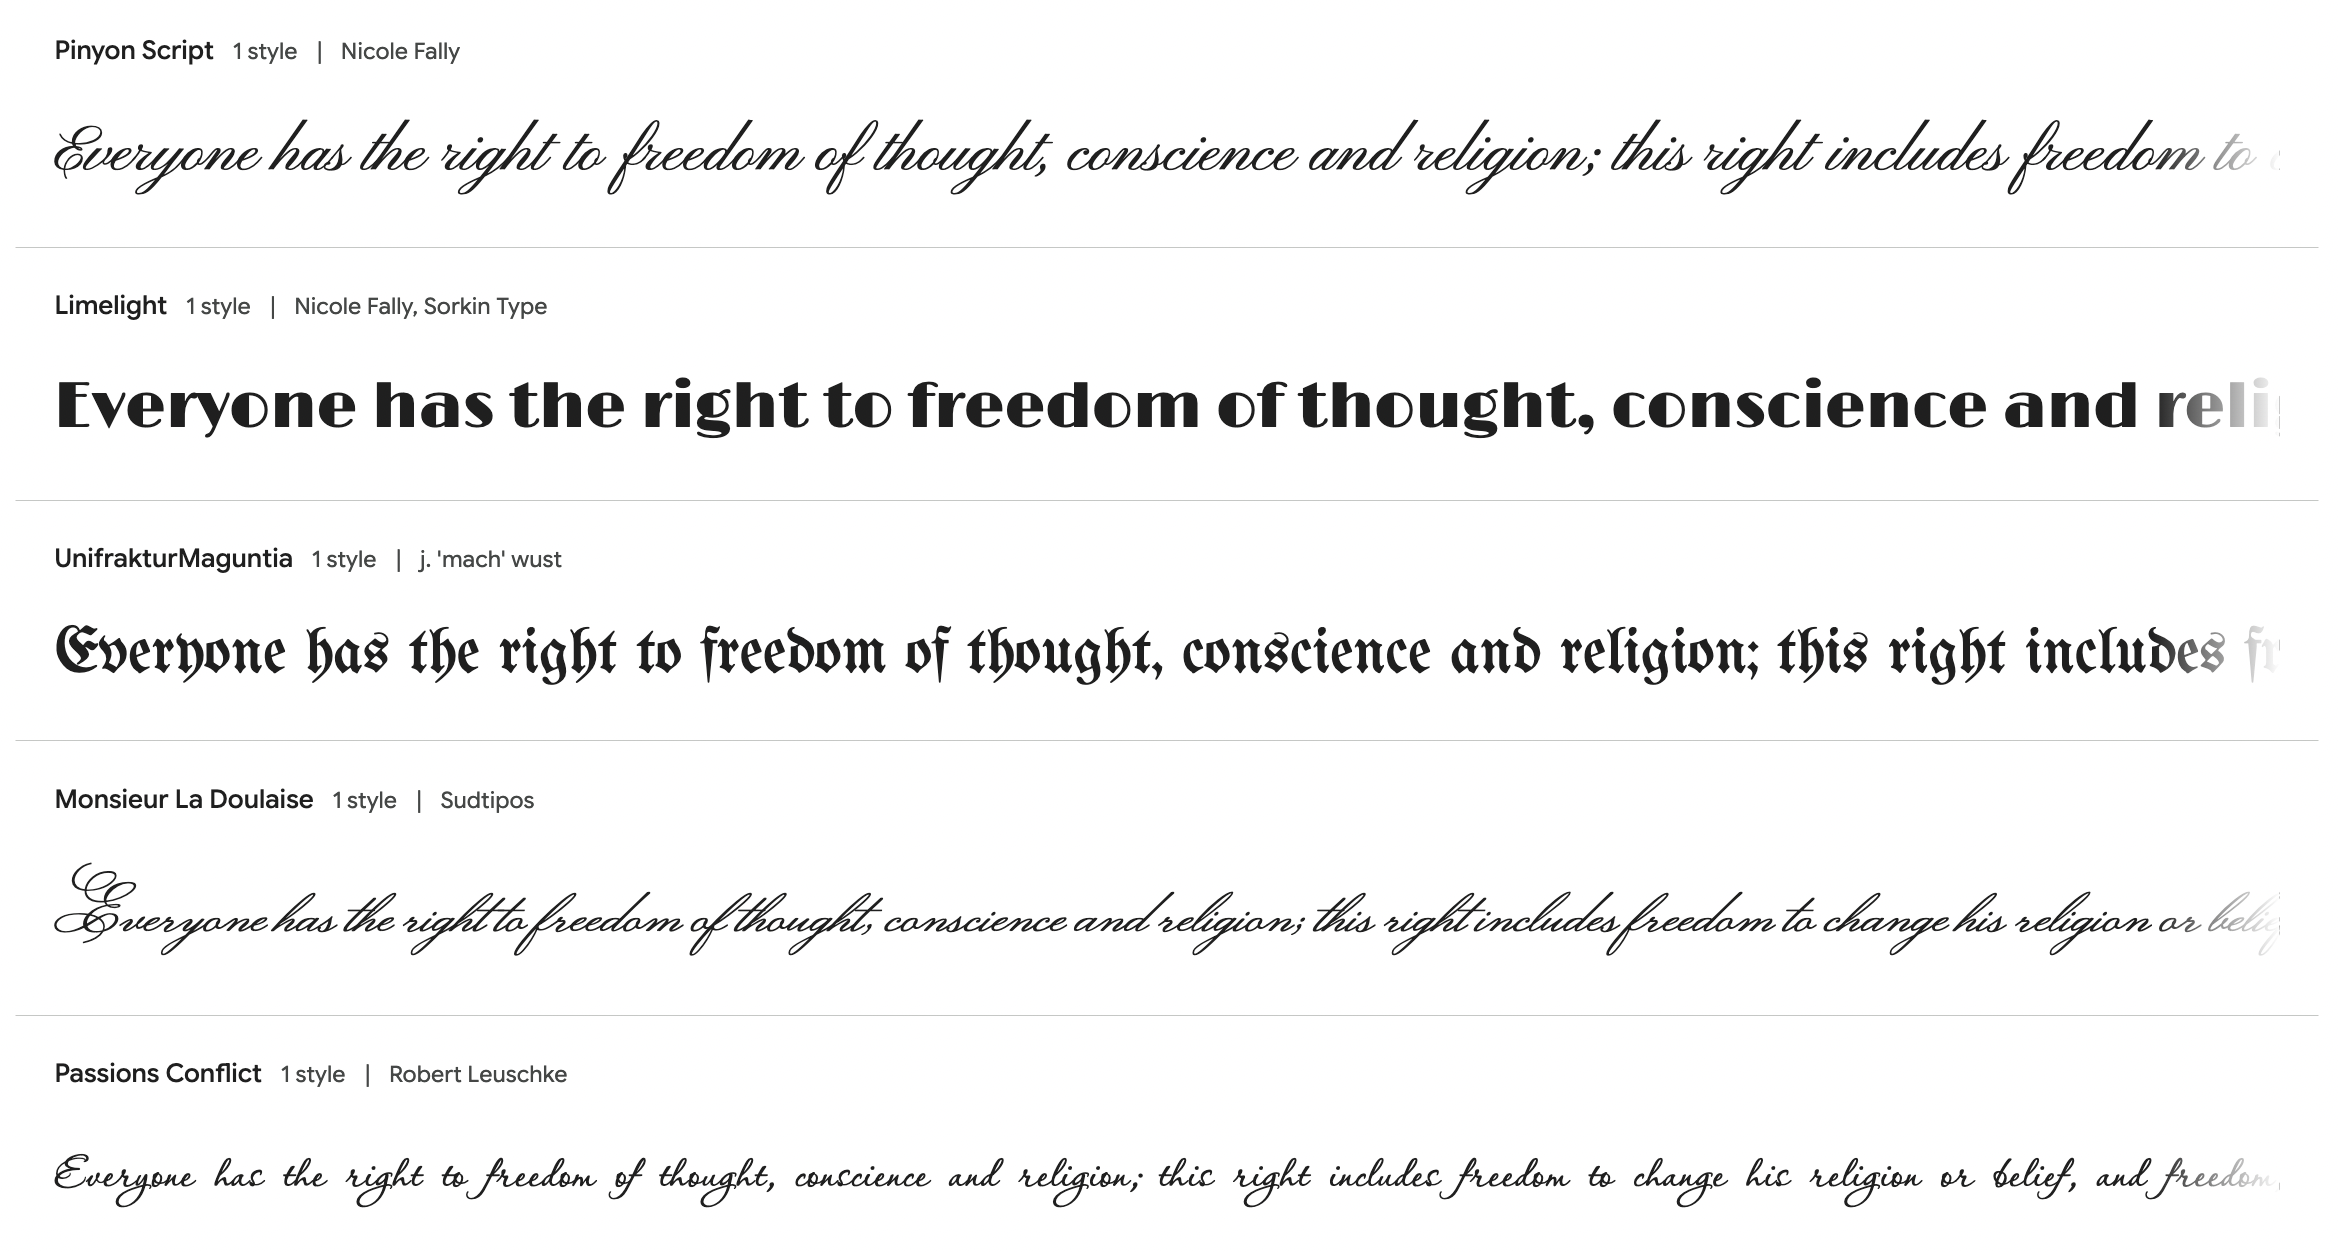
\includegraphics[width=\textwidth]{images/feeling-artistic.png}
    \caption{Selection of fonts in the Google Fonts feeling-artistic category}
    \label{fig:feeling-artistic}
\end{figure}

% my own figure
\begin{figure}[p]
    \centering
    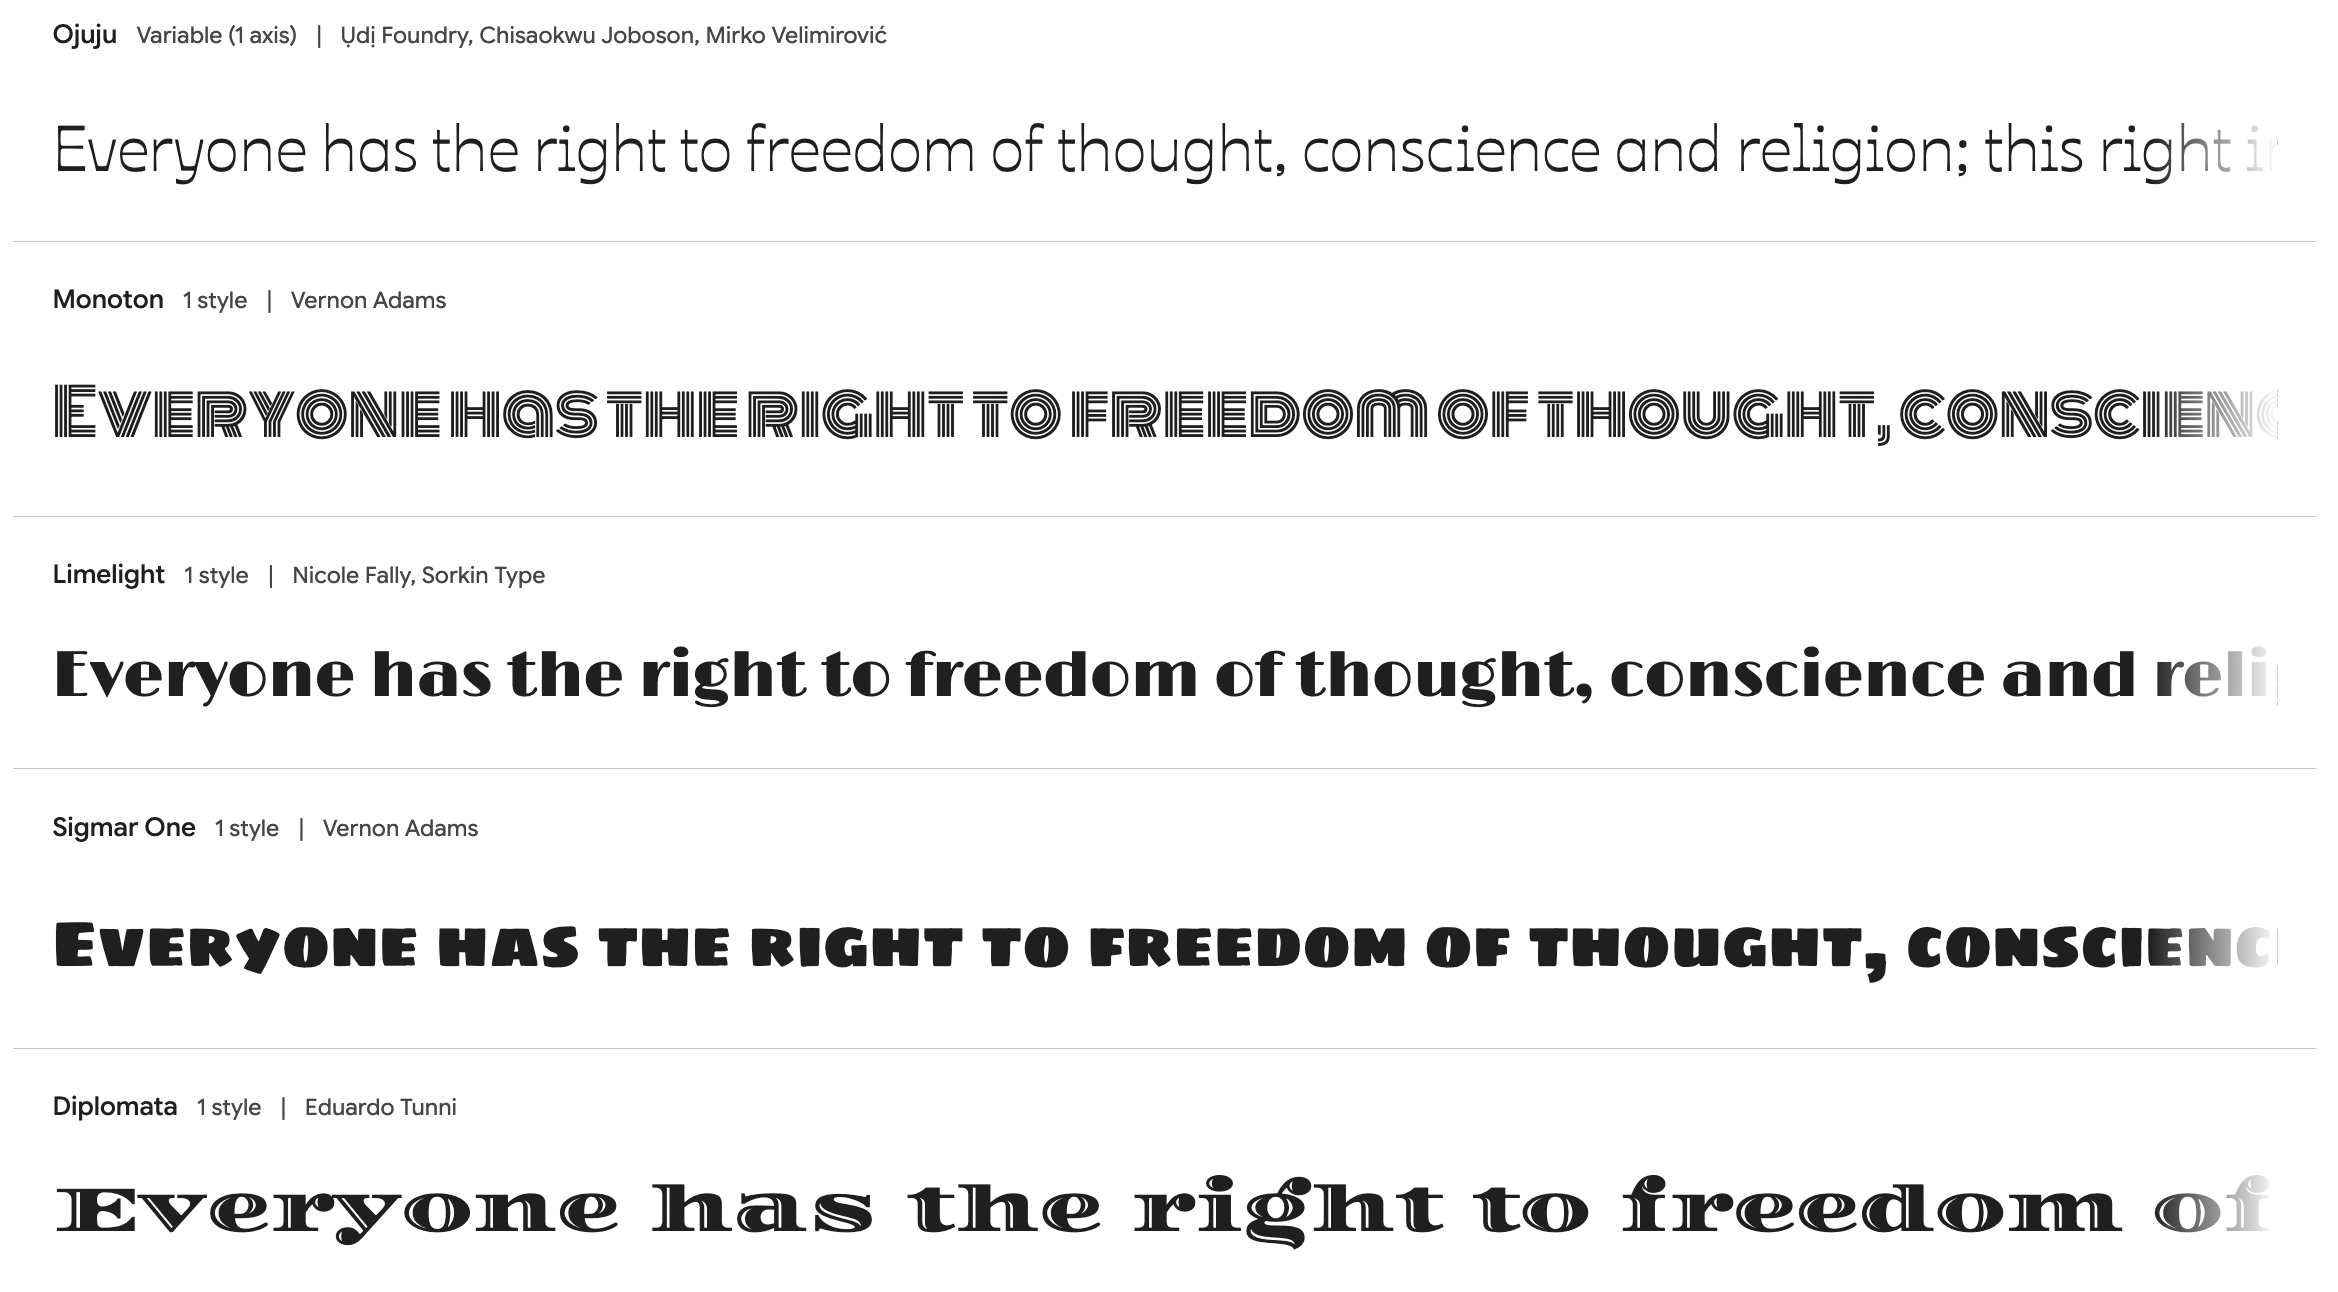
\includegraphics[width=\textwidth]{images/seasonal-kwanzaa.png}
    \caption{Selection of fonts in the Google Fonts seasonal-kwanzaa category}
    \label{fig:seasonal-kwanzaa}
\end{figure}

It makes sense that the Srivatsan model would perform better with our full dataset: partially, this may be due to simply having a larger, more representative training dataset; but this is also likely a result of having seen the Google Fonts in its training. In the latter instance, the Srivatsan model was able to actively optimize the style encodings for the Google Fonts typefaces, while the more limited Srivatsan model did not have the opportunity to specifically optimize these style encodings. This does not, however, mean that the Google Fonts style encodings of the full Srivatsan model are of lower quality; rather, having the ability to specifically train on these fonts should result in better, more accurate style encodings for use in our font selection tool.

Looking at the similarity scores across all the Google Fonts style categories (see Table \ref{tab:category-distances}), we can make some conclusions about the different models' abilities to encode certain types of style. For example, we find that all model implementations encode sans-serif style quite effectively, as the average distance scores for most of the sans-serif style groups are lower than the overall average distance in their model spaces. The same is true for most of the serif style groups; however, only the fully trained Srivatsan model seems capable of encoding the style of the serif-fatface and serif-slab groups. This makes some sense, as these two categories contain less typical serif style fonts (see Figures \ref{fig:serif-fatface} and \ref{fig:serif-slab}), but the groups are also relatively small (15 and 68 fonts, respectively) and it is hard to make a definite conclusion with such a small sample size.

We additionally find that some of the more ambiguous font style categories are not well-encoded by our simpler models. In particular, style categories in the appearance, feeling, and seasonal groups have low average similarity scores in the encoding spaces of the more basic models. For many of these ambiguous style categories, only the Srivatsan model trained on our full dataset seemed to recognize the implicit connections among their fonts. Many of these ambiguous stylistic categories contain a wide variety of different font styles, making it difficult to explicitly identify their common traits. For example, the fonts in the feeling-artistic and seasonal-kwanzaa categories (see Figures \ref{fig:feeling-artistic} and \ref{fig:seasonal-kwanzaa}) do not seem to follow one particular or obvious style. Somewhat surprisingly, our final model recognizes common threads among fonts even in these more abstract style groups, suggesting that these model encodings should provide a strong foundation for style-based font selection.

\subsection{Euclidean Distance vs Cosine Similarity}

We find an interesting result when comparing the cosine and Euclidean distances in our model evaluation. In general, we find that the models which perform strongly for Euclidean distance do not perform as well when considering cosine similarity; and conversely, the models which perform less well in terms of Euclidean closeness perform better with cosine similarity. For example, when comparing the normalized category-wise Euclidean distances and cosine similarities of the Autoencoder model (see Table \ref{tab:euclidean-vs-cosine-auto-short}), we find that a greater number of categories have a better-than-average similarity when considering cosine similarity ($n=41$) rather than Euclidean distance ($n=23$); and the average similarity score across all category groups is closer than average (1.125) as measured by cosine similarity but further than average (1.318) when using Euclidean distance. On the other hand, our full Srivatsan model performs very well on Euclidean distance scores but not as well when using cosine similarity (see Table \ref{tab:euclidean-vs-cosine-sriv-short}), with far fewer scores beating the average under the cosine similarity metric ($n=36$) and the average category-wise cosine similarity score (0.987) slightly worse than the overall pairwise average for the full model space. It is unclear exactly why there is a discrepancy with cosine and Euclidean similarity evaluation in our model space. It is certainly the case that Euclidean and cosine similarity metrics are measuring different types of vector similarity, which might be representing different aspects of the model encodings. However, for the purposes of our selection tool this should not matter. Since our user tool is built around Euclidean distance measurements, it is mainly important that our full Srivatsan model performs well under Euclidean distance metrics---that similar font styles should be closer to each other in Euclidean space---which it does. Cosine similarity metrics tell an interesting story about our model space, but ultimately the metric of most importance for our purposes is Euclidean distance.

\begin{longtable}{|l|r|r|}
\caption{Normalized average pairwise Euclidean and cosine distances across Google Fonts category groups in our Autoencoder model space. Distances closer than the overall pairwise average (less than one for Euclidean, greater than one for cosine) are bolded. Abbreviated from Table \ref{tab:euclidean-vs-cosine-auto} (Appendix).}
\label{tab:euclidean-vs-cosine-auto-short} \\
\hline
\textbf{Category} & \textbf{Autoencoder (Euclidean)} & \textbf{Autoencoder (Cosine)} \\
\hhline{|===|}
average category distance & 1.318 & \textbf{1.125} \\
\% categories beat average & 34.8\% & 62.1\% \\
\hhline{|===|}
\endfirsthead

\multicolumn{3}{c}{{Table \thetable\ continued from previous page}} \\[0.5em]
\hline
\textbf{Category} & \textbf{Autoencoder (Euclidean)} & \textbf{Autoencoder (Cosine)} \\
\hline
\endhead

\hline \multicolumn{3}{r}{{Continued on next page}} \\
\endfoot

\hline
\endlastfoot

appearance-art-deco       & 1.728                   & \textbf{1.282}      \\
appearance-art-nouveau    & \textbf{0.453}          & 0.494               \\
appearance-blackletter    & \textbf{0.698}          & \textbf{1.101}      \\
appearance-blobby         & 1.198                   & 0.906               \\
appearance-distressed     & 1.489                   & \textbf{1.434}      \\
appearance-inline         & 2.238                   & \textbf{1.692}      \\
appearance-lunar-new-year & 1.390                   & \textbf{1.742}      \\
appearance-marker         & 1.139                   & \textbf{1.045}      \\
appearance-medieval       & \textbf{0.934}          & 0.848               \\
appearance-monospaced     & \textbf{0.475}          & 0.866               \\
appearance-not-text       & 6.477                   & \textbf{2.699}      \\
\hline
\multicolumn{3}{|c|}{$\cdots$} \\
\hline
serif-didone              & 1.238                   & 0.853               \\
serif-fatface             & 2.478                   & 0.666               \\
serif-humanist            & \textbf{0.628}          & 0.535               \\
serif-modern              & \textbf{0.794}          & 0.955               \\
serif-old-style           & \textbf{0.522}          & 0.544               \\
serif-scotch              & \textbf{0.562}          & 0.808               \\
serif-slab                & 1.582                   & 0.920               \\
serif-transitional        & 0.551                   & 0.529         \\           

\end{longtable}

\begin{longtable}{|l|r|r|}
\caption{Normalized average pairwise Euclidean and cosine distances across Google Fonts category groups in our full Srivatsan model space. Distances closer than the overall pairwise average (less than one for Euclidean, greater than one for cosine) are bolded. Abbreviated from Table \ref{tab:euclidean-vs-cosine-sriv} (Appendix).}
\label{tab:euclidean-vs-cosine-sriv-short} \\
\hline
\textbf{Category} & \textbf{Srivatsan Full (Euclidean)} & \textbf{Srivatsan Full (Cosine)} \\
\hhline{|===|}
average category distance & \textbf{0.769} & 0.987 \\
\% categories beat average & 98.5\% & 54.5\% \\
\hhline{|===|}
\endfirsthead

\multicolumn{3}{c}{{Table \thetable\ continued from previous page}} \\[0.5em]
\hline
\textbf{Category} & \textbf{Srivatsan Full (Euclidean)} & \textbf{Srivatsan Full (Cosine)} \\
\hline
\endhead

\hline \multicolumn{3}{r}{{Continued on next page}} \\
\endfoot

\hline
\endlastfoot

appearance-art-deco       & \textbf{0.780}             & \textbf{1.266}          \\
appearance-art-nouveau    & \textbf{0.706}             & 0.650                   \\
appearance-blackletter    & \textbf{0.921}             & 0.881                   \\
appearance-blobby         & \textbf{0.657}             & 0.955                   \\
appearance-distressed     & \textbf{0.698}             & \textbf{1.303}          \\
appearance-inline         & \textbf{0.732}             & \textbf{1.140}          \\
appearance-lunar-new-year & \textbf{0.841}             & \textbf{1.264}          \\
appearance-marker         & \textbf{0.651}             & \textbf{1.104}          \\
appearance-medieval       & \textbf{0.758}             & 0.855                   \\
appearance-monospaced     & \textbf{0.746}             & 0.909                   \\
appearance-not-text       & \textbf{0.754}             & \textbf{1.707}          \\
\hline
\multicolumn{3}{|c|}{$\cdots$} \\
\hline
serif-humanist            & \textbf{0.841}             & 0.525                   \\
serif-modern              & \textbf{0.889}             & 0.597                   \\
serif-old-style           & \textbf{0.814}             & 0.477                   \\
serif-scotch              & \textbf{0.891}             & 0.502                   \\
serif-slab                & \textbf{0.845}             & 0.849                   \\
serif-transitional        & \textbf{0.954}             & 0.468              

\end{longtable}

\section{User Evaluation} \label{user-eval}

% my own figure
\begin{figure}[h]
    \centering
    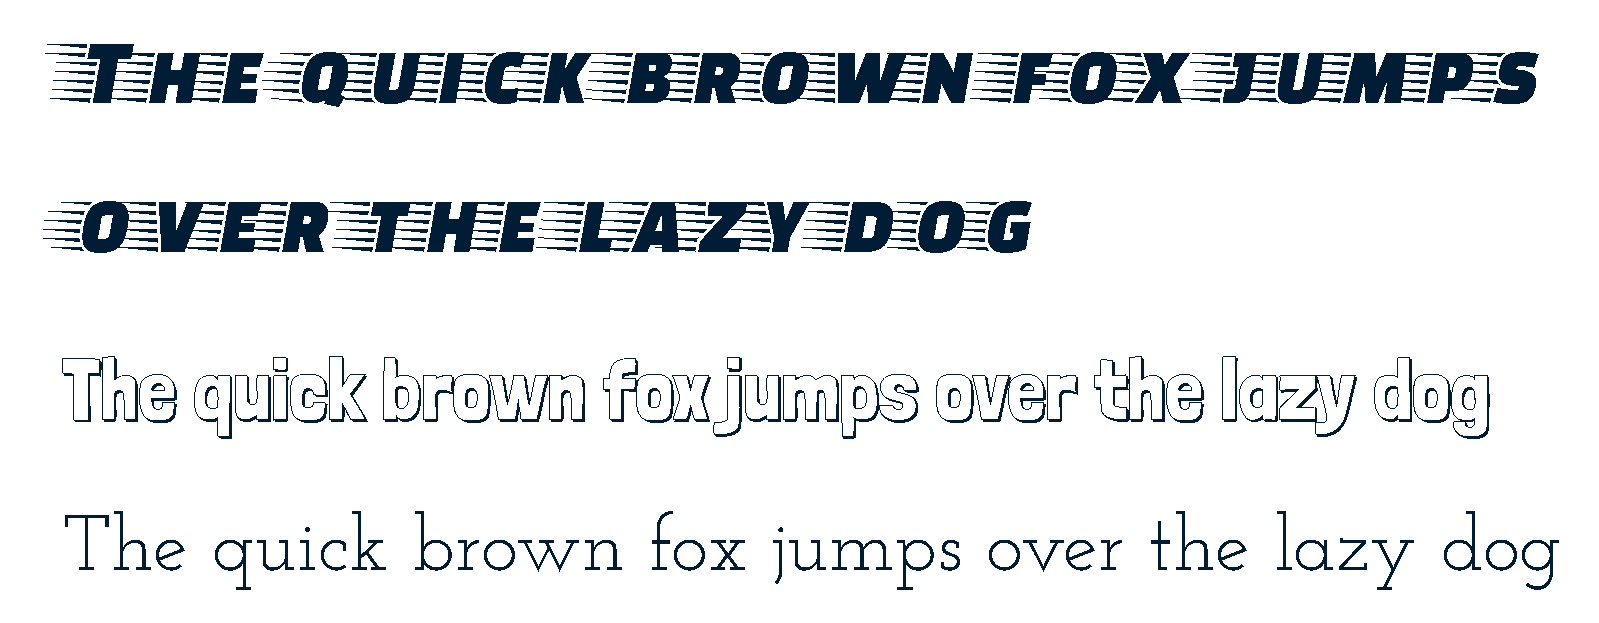
\includegraphics[width=\textwidth]{images/user-fonts.pdf}
    \caption{Fonts chosen for our user study (Faster One, Londrina Shadow, and Josefin Slab, from top to bottom) with sample text ``The quick brown fox jumped over the lazy dog''}
    \label{fig:user-fonts}
\end{figure}

We additionally conducted a small user study to qualify the effectiveness of our font selection interface. Our participants were 12 college students. Each of the 12 participants were given three fonts (on a printed piece of paper) and three corresponding font identification tasks using each of three interfaces: the basic list-based font selector in Google Docs, the category-based search from Google Fonts, and our typeface-space selector. We chose three fonts which represent a variety of search difficulties: one which was very distinct and would not be confused with another typeface in our set (Faster One), another which was somewhat distinct but has some lookalike fonts in the set (Londrina Shadow), and a third which was more generic and likely harder to find among similar fonts (Josefin Slab). For each user, we presented one of the three fonts showing a default display text (see Figure \ref{fig:user-fonts}) and introduced one of the tools. We then gave the participant two minutes to try and identify the font using the given tool. We repeated the task two additional times, randomizing the order of tools between participants, so that each user tried all three tools and attempted to identify each font. By randomizing tool order but keeping font order the same, we ensured that our performance data was not affected by the choice of font. We kept track of several metrics: remaining time (if the user selected a font in less than two minutes); \# of clicks, mouse movements, and scrolls; and also the selected font, which we used to calculate the normalized Euclidean distance from the correct font in our model space (i.e. how close the user got, zero if correct) as well as percent accuracy.

\begin{longtable}{|l|r|r|r|r|r|r|}
\caption{Quantitative results from font matching user study, averaged across trials, with distance from correct normalized to average pairwise distance in encoding space.}
\label{tab:user-study-quant} \\
\hline
\textbf{selector} & \textbf{\% correct} & \textbf{distance} & \textbf{time left} & \textbf{clicks} & \textbf{scrolls} & \textbf{mouse moves} \\
\hline
\endfirsthead

\multicolumn{3}{c}{{Table \thetable\ continued from previous page}} \\[0.5em]
\hline
\textbf{selector} & \textbf{\% correct} & \textbf{distance} & \textbf{time left} & \textbf{clicks} & \textbf{scrolls} & \textbf{mouse moves} \\
\hline
\endhead

\hline \multicolumn{3}{r}{{Continued on next page}} \\
\endfoot

\hline
\endlastfoot

list & 0.5 & 0.353 & 0:30 & 8.9 & 72 & 60.4 \\
google fonts & 0.67 & 0.291 & 0:29 & 16.2 & 62.5 & 78.9 \\
our tool & 0.55 & 0.359 & 0:39 & 23.6 & 2.9 & 112.6                 

\end{longtable}

Table \ref{tab:user-study-quant} shows the quantitative results from our user study. Given the small size of the study ($n=12$) and the many possible sources of noise in our trial, it is difficult to draw many significant conclusions from our data. For example, it appears as though users chose slightly closer-to-correct fonts (according to the Euclidean distance metric in our encoding space) when using the Google Fonts selector---and were also more often correct in their selection---but given the closeness of these numbers and the high amount of variation in our data, we cannot substantially differentiate these performances. The data that appear most significant are our measures of clicks, scrolls, and mouse moves: unsurprisingly, users tended to scroll more on the basic list and Google Fonts selectors---which are both scroll-based interfaces---and tended to use more mouse moves on our tool, which relies on mouse movements for most of its selection mechanisms. While the study was too small to make significant conclusions about accuracy performance, it is useful to explore methods for quantifying font selection tools and begin to understand the usefulness of our tool. Importantly, a font matching task may not be the best method to evaluate tool performance, as oftentimes in real-world use scenarios, users do not seek to match an exact font but rather to explore several fonts and find a desireable one. O'Donovan et al. \cite{odonovan2014}, for example, utilize two tasks in their font selection tool evaluation: a font matching task similar to ours, and also a more subjective task asking to find a ``good'' font for the design of a given document.

At the end of each trial, we also asked users to qualitatively evaluate each of the tools. For each selector, we simply asked the user to list positive and negative aspects of each tool---what they liked, didn't like, found helpful, or not. These results are helpful in both evaluating our own tool and better understanding user needs in font selection tasks. Table \ref{tab:user-study-qual} shows a summary of user responses, organized by ``advantages'' and ``disadvantages'' of each tool. For the basic list interface, we received the same piece of feedback from most users: that alphabetical order is not useful when selecting fonts based on style, and the lack of categories led to a long, mundane search experience. Additionally, users reported finding the small text size difficult and found it frustrating that the tool did not save their place in the long list when they clicked away from it. However, users did find the simplicity of the interface useful, as well as the fact that it displays many characters at once in the font name. For the Google Fonts category-search interface, users liked the ability to search by attribute, but they found that the categories were often too vague or subjective; additionally, sometimes a category they envisioned and hoped to use (e.g. ``Block Letters'') was not an available option. For our style-based tool, users liked that the interface tended to cluster fonts by similarity, allowing them to narrow down their search and eliminate parts of the map from consideration, and generally found the interface to be fun and explorative; however, many found the tool somewhat unintuitive and difficult to use at first, wished they could preview more letters at once, and were frustrated by the lag which occurs due to character re-rendering when zooming in the map tool.

\begin{longtable}{|l|l|l|}
\caption{Summary of qualitative results from user study, separated into ``advantages'' and ``disadvantages'' of each tool.}
\label{tab:user-study-qual} \\
\hline
& \textbf{advantages} & \textbf{disadvantages} \\
\hline
\endfirsthead

\multicolumn{3}{c}{{Table \thetable\ continued from previous page}} \\[0.5em]
\hline
& \textbf{advantages} & \textbf{disadvantages} \\
\hline
\endhead

\hline \multicolumn{3}{r}{{Continued on next page}} \\
\endfoot

\hline
\endlastfoot

list &

\begin{tabular}[c]{@{}l@{}}
simple interface\\
helpful if you know the name already\\
ability to save fonts\\
displays many letters for each font
\end{tabular} &

\begin{tabular}[c]{@{}l@{}}
no style-based search\\
alphabetic order is not useful\\
too much to scroll through\\
doesn't save your place\\
small text\\
boring
\end{tabular} \\

google fonts &

\begin{tabular}[c]{@{}l@{}}
ability to preview text\\
search by attribute\\
ability to narrow down search
\end{tabular} &

\begin{tabular}[c]{@{}l@{}}
categories are subjective and often vague\\
too many categories\\
some categories did not exist\\
no open-ended descriptor search
\end{tabular}\\

\hline

our tool &

\begin{tabular}[c]{@{}l@{}}
ability to narrow down search\\
clustered by similarity\\
ability to eliminate areas of map from\\
search based on style\\
playful interface\\
fun to explore
\end{tabular} &

\begin{tabular}[c]{@{}l@{}}
difficult to understand many features\\
dimensional aspect unclear\\
font not always where expected\\
only able to display one letter\\
lag with character rendering\\
no text-based search feature
\end{tabular} \\

\end{longtable}

These qualitative data are useful in understanding how users make use of our tool and evaluating it against other existing font selection interfaces. For example, there was a clear sentiment, expressed by almost all of our participants, that the basic list selector was limited by not including any aspect of style or stylistic categories in its interface. Users tended to like the Google Fonts category search, but the subjectivity of categories was a limiting factor. Our style-encoding search represents a very different method of font selection: one based on trained, quantitative stylistic model encodings. While our tool was somewhat unintuitive for some first-time users, it was nonetheless received well as a fun and useful style-based font exploration tool. Some improvements would be necessary to make this into a finalized user-ready tool, but this proof-of-concept font selection interface suggests that the style encodings produced by autoencoder-like neural networks can certainly be used to create useful style-based typeface selection tools.